\documentclass{article}
\usepackage[utf8]{inputenc}
\textheight = 25cm 
\textwidth = 15cm
\topmargin = -2.5cm 
\oddsidemargin = 1.5cm
\usepackage{float}
\usepackage{graphicx}
\graphicspath{{./images/}}

\usepackage{amsmath}
\usepackage{mathtools, xparse}
\usepackage[shortlabels]{enumitem}
\usepackage[most]{tcolorbox}
\usepackage{adjustbox}
\usepackage{bm} 

\DeclarePairedDelimiter{\norm}{\lVert}{\rVert}

\title{Tarea 5 Mecánica Analítica}
\author{Cerritos Lira Carlos}
\date{18 de Marzo del 2020}

\begin{document}
\maketitle
\section*{Problemas}
\subsection*{1.- }
Calcule la desviación de la plomada en el hemisferio sur.
\begin{tcolorbox}
    Consideremos dos sistemas de referencia, $S$ en el centro de la tierra y $S'$ en la superficie de la Tierra orientado como en el dibujo:
    \begin{figure}[H]
        \centering
        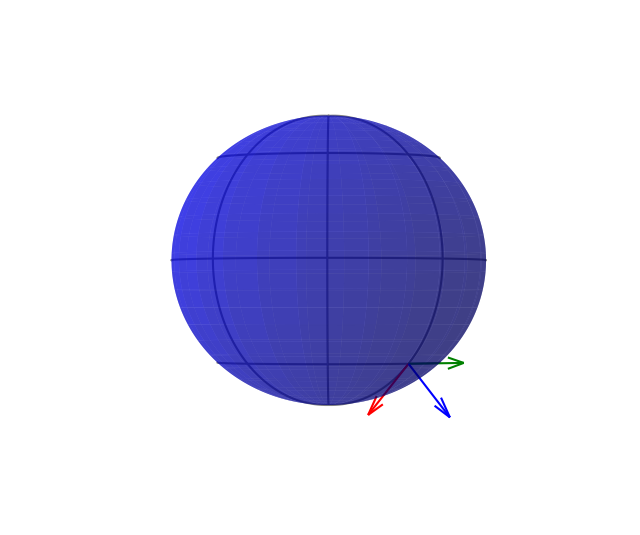
\includegraphics[scale=0.5, trim=50 50 50 50, clip]{p1_world}
        \caption{Sistema de referencia $S'$}
        \label{fig:galaxy}
    \end{figure}
    \begin{figure}[H]
        \centering
        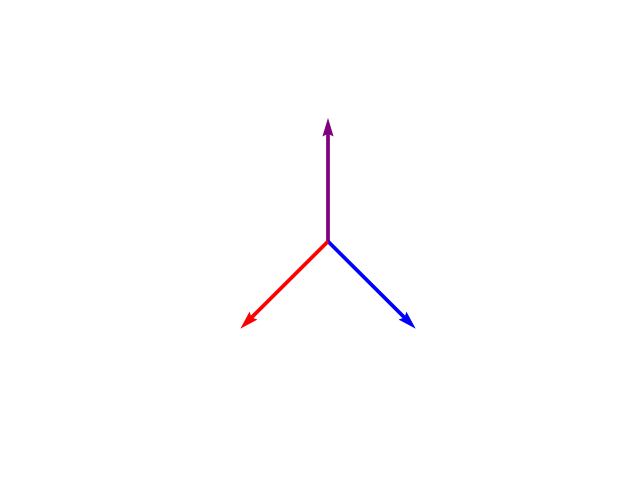
\includegraphics[scale=0.5, trim=60 60 60 60, clip]{p1_axis}
        \caption{Relación entre vectores $\bm{\Omega, i, k}$}
        \label{fig:my_label}
    \end{figure}
    sabemos que se cumple la relación:
    \begin{align*}
        \frac{d^2\bm{r}}{dt^2}  
        &=\frac{d^2(\bm{r' + R'})}{dt^2}
        + 2\bm{\Omega} \times \frac{d(\bm{r' + R'})}{dt}
        + \bm{\Omega} \times (\bm{\Omega} \times (\bm{r' + R'})) \\
    \end{align*}
    \end{tcolorbox}
\begin{tcolorbox}
    usando las condiciones del problema:
    \begin{align*}
        \bm{R'} &= R\bm{k} \\
        \frac{d^2\bm{r}}{dt^2} &= -g\bm{k}
    \end{align*}
    quitando los términos que se hacen cero o son muy pequeños obtenemos la relación:
    \begin{align*}
        \frac{d^2\bm{r'}}{dt^2}
        &= \frac{d^2\bm{r}}{dt^2} - \bm{\Omega} \times (\bm{\Omega} \times \bm{R'}) \\
        &= \bm{g} - \bm{a_c}
    \end{align*} 
    escribimos a $\bm{\Omega}$ como combinación lineal de $\bm{i,k}$:
    \begin{align*}
        \frac{\bm{\Omega}}{\Omega} 
        &= cos(\pi - \lambda)\bm{i} + cos\left(\frac{\pi}{2} - \lambda \right) \bm{k} \\
        \frac{\bm{\Omega}}{\Omega} 
        &= -cos\lambda \bm{i} + sin\lambda \bm{k} \\
        \frac{\bm{\Omega} \times \bm{R'}}{\Omega R}
        &= cos\lambda \bm{j} \\
        \frac{\bm{\Omega} \times (\bm{\Omega} \times \bm{R'})}{\Omega^2 R}
        &= -cos^2\lambda \bm{k} - sin\lambda cos\lambda \bm{i} 
    \end{align*}
    sustituyendo obtenemos la aceleración:
    \begin{align*}
        \frac{d^2\bm{r'}}{dt^2} 
        &= \bm{g} - \bm{a_c} \\ 
        &= -g\bm{k} + \Omega^2R cos^2\lambda \bm{k} + \Omega^2 R sin\lambda cos\lambda \bm{i}
    \end{align*}
    procedemos a encontrar el ángulo entre $\bm{g}$ y $\bm{g_{real}}$
    \begin{align*}
        cos\theta
        &=\frac{\bm{g}}{g} \cdot \frac{\bm{g-a_c}}{\Omega^2 R} \\
        &=\frac
        {\frac{g}{\Omega^2 R} - cos^2\lambda}
        {((\frac{g}{\Omega^2 R})^2 + cos^4\lambda + sin^2\lambda cos^2\lambda)^{1/2}} \\
        &=\frac
        {\frac{g}{\Omega^2 R} - cos^2\lambda}
        {((\frac{g}{\Omega^2 R})^2 + cos^2\lambda)^{1/2}} \\ 
    \end{align*}
    se puede ver un resultado esperado, esto es, cuando $\lambda = \frac{\pi}{2}$, se tiene $\theta = 0$
\end{tcolorbox}
\subsection*{2.- }
Calcule la magnitud y la dirección de la desviación de la caída
libre en el hemisferio sur.
\begin{tcolorbox}
    Definimos nuevamente dos sistemas de referencia, $S$ en el centro del planeta y $S'$ como en la figura 1. \\
    Sabemos que se cumple la relación: 
    \begin{align*}
        \frac{d^2\bm{r}}{dt^2}  
        &=\frac{d^2(\bm{r' + R'})}{dt^2}
        + 2\bm{\Omega} \times \frac{d(\bm{r' + R'})}{dt}
        + \bm{\Omega} \times (\bm{\Omega} \times (\bm{r' + R'})) \\
    \end{align*}
    \end{tcolorbox}
    \begin{tcolorbox}
    usamos las condiciones del problema:
    \begin{align*}
        \bm{R'} &= R\bm{k} \\
        \frac{d^2\bm{r}}{dt^2} &= -g\bm{k} 
    \end{align*}
    ignorando la aceleración centrípeta obtenemos la relaciones:
    \begin{align*}
        \frac{d^2\bm{r'}}{dt^2}
        &= \frac{d^2\bm{r}}{dt^2} - 2\bm{\Omega} \times \frac{d\bm{r'}}{dt} \\
        &= \bm{g} - 2\bm{\Omega} \times \frac{d\bm{r'}}{dt} \\
        \frac{d\bm{r'}}{dt}
        &= (t-t_0)\bm{g} - 2\bm{\Omega} \times (\bm{r'} - \bm{r_0'}) + \bm{v_0'} \\
        \bm{r'}
        &= \frac{(t-t_0)^2}{2}\bm{g} + (t-t_0)\bm{v_0'} - \int_{t_0}^t 2\bm{\Omega} \times (\bm{r'} - \bm{r_0'}) + \bm{r_0'} \\
        &= \frac{(t-t_0)^2}{2}\bm{g} + (t-t_0)\bm{v_0'} - 2\bm{\Omega} \times \int_{t_0}^t \bm{r'} + 2(t-t_0)\bm{\Omega} \times \bm{r_0'} + \bm{r_0'} 
    \end{align*}
    aproximamos el valor de $\bm{\Omega} \times \bm{r'}$:
    \begin{align*}
        \bm{\Omega} \times \bm{r'}
        &= \bm{\Omega} \times 
        \left[ \frac{(t-t_0)^2}{2}\bm{g} + (t-t_0)\bm{v_0'} - 2\bm{\Omega} \times \int_{t_0}^t \bm{r'} + 2(t-t_0)\bm{\Omega} \times \bm{r_0'} + \bm{r_0'} \right] \\
        &= \bm{\Omega} \times 
        \left[ \frac{(t-t_0)^2}{2}\bm{g} + (t-t_0)\bm{v_0'} + \bm{r_0'} \right]
    \end{align*}
    sustituyendo encontramos expresión analítica de $\frac{d\bm{r'}}{dt}$:
    \begin{align*}
        \frac{d\bm{r'}}{dt}
        &=(t-t_0)\bm{g} - 2\bm{\Omega} \times 
        \left[ \frac{(t-t_0)^2}{2}\bm{g} + (t-t_0)\bm{v_0'} \right] + \bm{v_0'} \\
        \bm{r'}
        &=\left[ (t-t_0) - (t-t_0)^2\bm{\Omega} \times \right] \bm{v_0'} 
        + \left[ \frac{(t-t_0)^2}{2} - \frac{(t-t_0)^3}{3} \bm{\Omega} \times \right]\bm{g} \\
        &=\left[ \frac{(t-t_0)^2}{2} - \frac{(t-t_0)^3}{3} \bm{\Omega} \times \right]  \bm{g} 
    \end{align*}
    si definimos $\bm{d} = -\frac{(t-t_0)^3}{3} \bm{\Omega} \times \bm{g}$ se tiene:
    \begin{align*}
        \bm{d} 
        &=-\frac{(t-t_0)^3}{3} \bm{\Omega} \times \bm{g} \\
        &=\frac{g(t-t_0)^3}{3} g\Omega(-cos\lambda\bm{i} + sin\lambda \bm{k}) \times \bm{k} \\
        &=\frac{(t-t_0)^3}{3} g\Omega cos\lambda \bm{j}
    \end{align*}
    de donde obtenemos $\bm{r'}$:
    \begin{align*}
        \bm{r'} 
        &= \frac{(t-t_0)^2}{2} \bm{g} + \bm{d} \\
        &= -\frac{(t-t_0)^2}{2} g\bm{k} + \frac{(t-t_0)^3}{3} g\Omega cos\lambda \bm{j} 
    \end{align*}
    obtenemos un resultado esperado, la fuerza centrifuga es la mismas latitudes pero 
    diferentes hemisferios. \\  
\end{tcolorbox}

\subsection*{3.- }
Calcule la magnitud y la dirección de la desviación del tiro vertical
en el hemisferio norte
\begin{tcolorbox}
    Tomemos dos sistemas de referencia, $S$ en el centro del planeta y $S'$ como en la figura 1. \\ 
    En el problema 1 vimos que $\bm{\Omega}$ tiene los mismos coeficientes en la combinación lineal 
    para ambos hemisferios. \\
    Del problema 2 tenemos la relación
    \begin{align*}
        \bm{r'}
        &=\left[ (t-t_0) - (t-t_0)^2\bm{\Omega} \times \right] \bm{v_0'} 
        + \left[ \frac{(t-t_0)^2}{2} - \frac{(t-t_0)^3}{3} \bm{\Omega} \times \right]\bm{g} \\
        &=(t-t_0)\bm{v_0'} + \frac{(t-t_0)^2}{2}\bm{g}
        - \bm{\Omega} \times \left[ (t-t_0)^2\bm{v_0'} + \frac{(t-t_0)^3}{3}\bm{g} \right] \\
        &=(t-t_0)\bm{v_0'} + \frac{(t-t_0)^2}{2}\bm{g} + \bm{d}
    \end{align*}
    desarrollamos $\bm{d}$
    \begin{align*}
        \bm{d}
        &=-\bm{\Omega} \times \left[ (t-t_0)^2\bm{v_0'} + \frac{(t-t_0)^3}{3}\bm{g} \right] \\
        &=-\bm{\Omega} \times \left[ (t-t_0)^2v_0' - \frac{(t-t_0)^3}{3}g \right] \bm{k} \\ 
        &=-\left[ (t-t_0)^2v_0' - \frac{(t-t_0)^3}{3}g \right]\Omega cos\lambda \bm{j}
    \end{align*}
    encontramos un resultado intuitivo, a medida que nuestro objeto sube observamos una fuerza
    lo desvia en la dirección $\bm{-j}$.   
\end{tcolorbox}

\subsection*{4.- }
Encontrar las velocidades y las aceleraciones de las partículas $p_1$ y $p_2$
del péndulo doble representando en la figura $3-17$: a) cuando el movimiento está 
confinado a un plano vertical (expresar $\bm{v}$ y $\bm{a}$ en función de 
$\theta_1, \theta_2, \dot{\theta_1}, \dot{\theta_2}$, etc)
\begin{tcolorbox}
    \begin{figure}[H]
        \centering 
        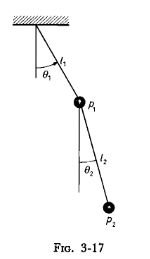
\includegraphics[scale=0.8]{p4-pendulo.png}
        \caption{Péndulo doble, movimiento contenido en un plano}
    \end{figure}
    Consideremos nuevos vectores para describir el movimiento 
    $\bm{e_{\theta_1}, e_{\theta_2}}$, llamemos $\bm{x_1, x_2}$ a las funciones que nos 
    dan la posición de las respectivas partículas en un tiempo $t$, se tiene la relación:
    \begin{align*}
        \bm{x_1} &= l_1\bm{e_{\theta_1}} \\
        \bm{x_2} &= \bm{x_1} + l_2\bm{e_{\theta_2}}  
    \end{align*}
\end{tcolorbox}
\begin{tcolorbox}
hacemos analisis para $\bm{e_{\theta_1}}$:
\begin{align*}
    \bm{e_{\theta_1}} 
    &= sin\theta_1 \bm{i} - cos\theta_1 \bm{j} \\
    \bm{\dot{e_{\theta_1}}} 
    &= \dot{\theta_1} (cos\theta_1 \bm{i} + sin\theta_1 \bm{j})\\
    &= \dot{\theta_1} \bm{e_{\phi_1}} \\
    \bm{\dot{e_{\phi_1}}}
    &= \dot{\theta_1} (-sin\theta_1 \bm{i} + cos\theta_1 \bm{j}) \\
    &= -\dot{\theta_1} \bm{e_{\theta_1}} 
\end{align*}
para $\bm{e_{\theta_1}}$ se cumplen las mismas relaciones, esto es:
\begin{align*}
    \bm{\dot{e_{\theta_2}}} 
    &= \dot{\theta_2} \bm{e_{\phi_2}} \\
    \bm{\dot{e_{\phi_2}}}
    &= -\dot{\theta_2}\bm{e_{\theta_2}}
\end{align*}
haciendo calculos encontramos:
\begin{align*}
    \bm{v_1} 
    &= l_1\dot{\theta_1}\bm{e_{\phi_1}} \\
    \bm{v_2} 
    &= \bm{v_1} + l_2\dot{\theta_2}\bm{e_{\phi_2}} \\
    \bm{a_1}
    &= l_1(\ddot{\theta_1}\bm{e_{\phi_1}} - \dot{\theta_1}^2\bm{e_{\theta_1}}) \\
    \bm{a_2}
    &= \bm{a_1} + l_2(\ddot{\theta_2}\bm{e_{\phi_2}} - \dot{\theta_2}^2\bm{e_{\theta_2}})
\end{align*}
las cuales son las relaciones que buscamos.
\end{tcolorbox}

\subsection*{5.-}
Se lanza un bloque hacia arriba sobre un plano inclinado con una velocidad inicial 
$v_0$. Si el plano forma un ángulo $\theta$ con la horizontal y el coeficiente de 
rozamiento(deslizante) entre el plano y el bloque es $\mu$, hallése el tiempo que
tarda el bloque en volver al pie del plano inclinado. ¿Cuál será el valor mínimo 
del coficiente de rozamiento en resposo o estático para que el bloque se detenga 
en el plano inclinado?
\begin{tcolorbox}
    Diagrama de fuerzas del problema:
    \begin{figure}[H]
        \centering 
        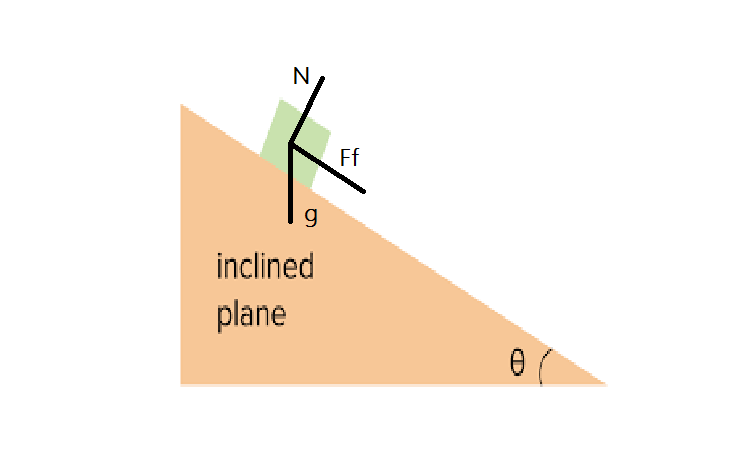
\includegraphics[scale=0.4]{p5_plano}
        \caption{Diagrama problema plano inclinado con velocidad inicial}   
    \end{figure}
\end{tcolorbox}
\begin{tcolorbox}
    Encontramos que la fuerza que actua en el objecto es
    \begin{align*}
        \frac{\bm{F}}{m} &=-g(\mu cos\theta + sin\theta) \bm{i}
    \end{align*}
    de donde obtenemos $\bm{x,v}$ la posición y velocidad en function del tiempo:
    \begin{align*}
        \bm{v} &=(v_0 - tg(\mu cos\theta + sin\theta)) \bm{i} \\
        \bm{x} &=(tv_0 -\frac{t^2}{2}g(\mu cos\theta + sin\theta))\bm{i}
    \end{align*}
    encontramos el tiempo de ascenso $t_a$, usando la condición $\bm{v} = 0$
    \begin{align*}
        t_a &= \frac{v_0}{g(\mu cos\theta + sin\theta)} \\
        \bm{x}(t_a) 
        &= \left[\frac{v_0^2}{g(\mu cos\theta + sin\theta)} - \frac{v_0^2}{2g(\mu cos\theta + sin\theta)} \right] \bm{i} \\
        &= \frac{v_0^2}{g(\mu cos\theta + sin\theta)} \bm{i} \\
        &= x_a\bm{i}
    \end{align*}
    ahora bien, una ves se detiene las fuerzas que actuan en el objeto son:
    \begin{align*}
        \frac{\bm{F}}{m} &= g(\mu cos\theta-sin\theta)\bm{i}
    \end{align*}
    de donde obtenemos $\bm{x,v}$ para $t \ge t_a$:
    \begin{align*}
        \bm{v} 
        &= (t-t_a)g(\mu cos\theta-sin\theta)\bm{i} \\
        \bm{x} 
        &= (x_a + \frac{(t-t_a)^2}{2}g(\mu cos\theta-sin\theta))\bm{i}
    \end{align*}
    encontramos el tiempo de descenso $t_d$, usando la condición $\bm{x}(t_d + t_a) = \bm{0}$
    \begin{align*}
        t_d^2 
        &= -\frac{x_a}{g(\mu cos\theta - sin\theta)} \\
        &= -\frac{v_0^2}{g(\mu cos\theta + sin\theta)g(\mu cos\theta - sin\theta)} \\
        &= \frac{v_0^2}{g^2(sin^2\theta - \mu^2cos^2\theta)} \\
        t_d 
        &= \sqrt{\frac{v_0^2}{g^2(sin^2\theta - \mu^2cos^2\theta)}} 
    \end{align*}
    el tiempo que tarda el bloque en volver es entonces:
    \begin{align*}
        t = t_a + t_d
    \end{align*}
    para que el bloque se detenga se debe de cumplir $\bm{v}(t_a + t_d) = \bm{0}$, de donde 
    obtenemos la condición:
    \begin{align*}
        \mu_{min} &= tan\theta
    \end{align*}
\end{tcolorbox}

\end{document}
